\chapter{Supplementary materials for:\\Large scale relationship between aquatic insect traits and climate}
\label{appendixC}

\section{Supplementary figures}
\label{Supplementary figures}

See next page.

\newpage

\begin{figure*}[hp!]
  \centering
  \hspace{-2cm} 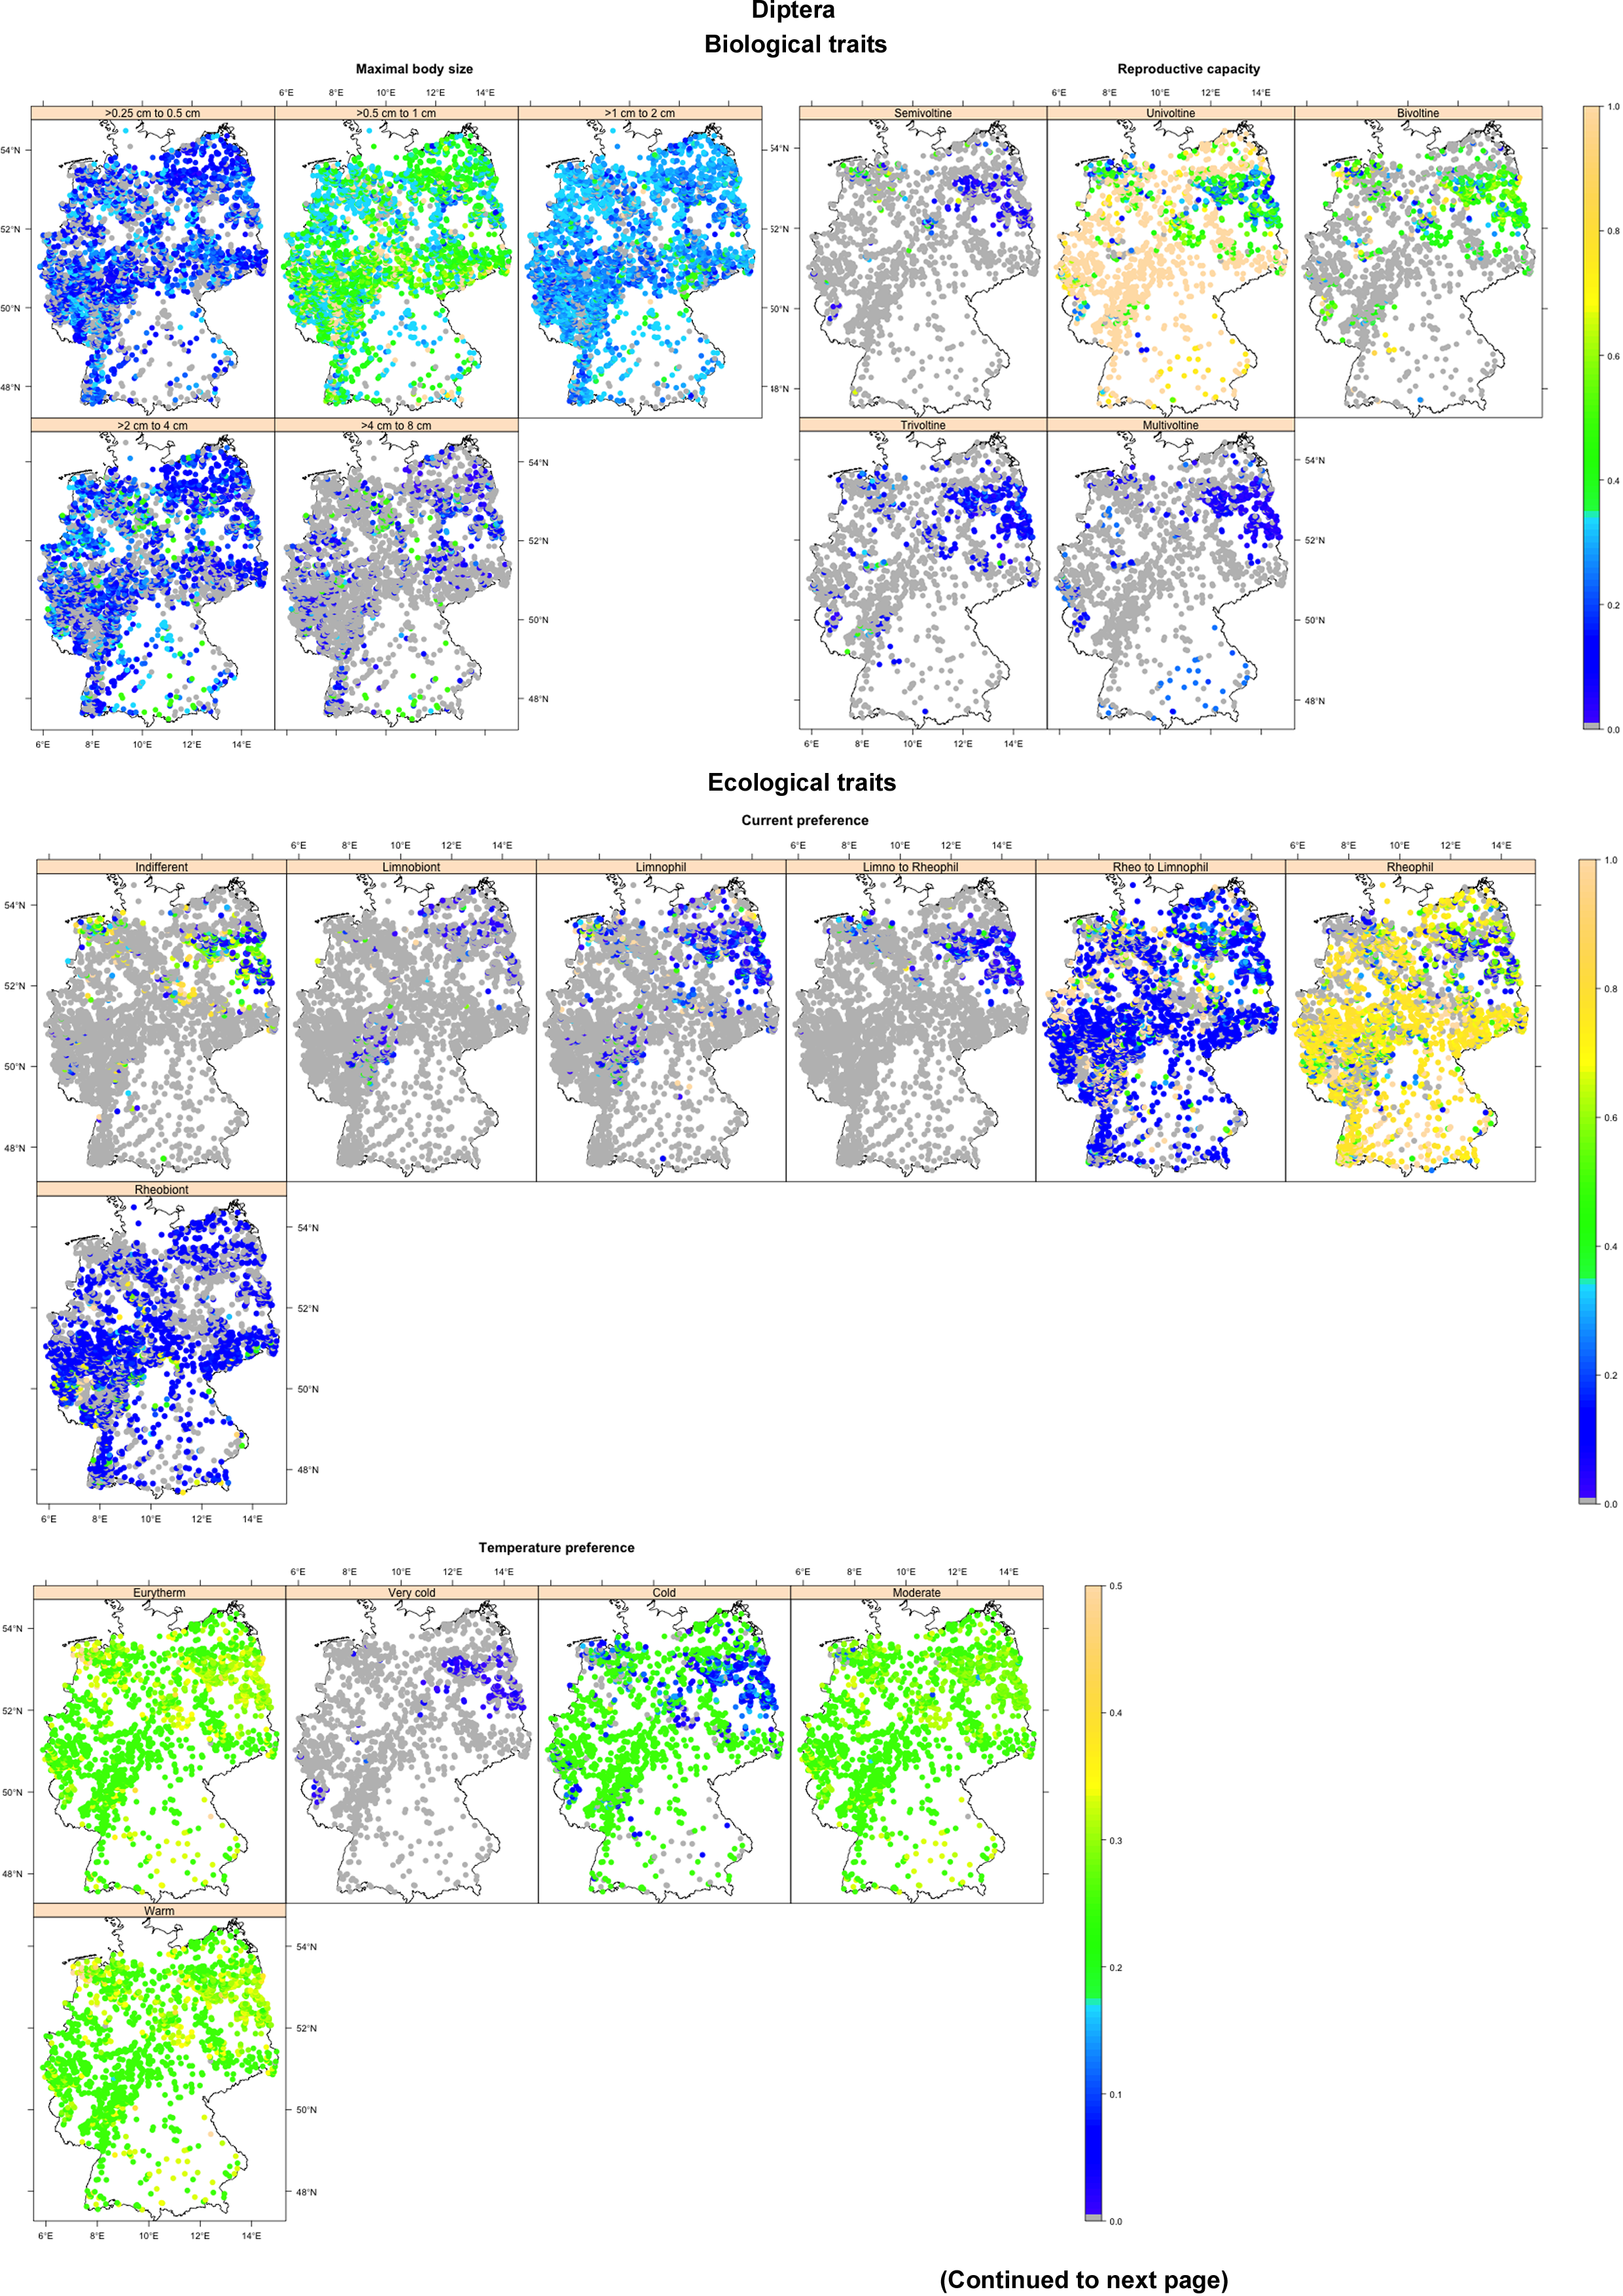
\includegraphics[width=1.1\textwidth]{Figures/Fig_C_1_a.png}
  \label{Fig_C_1_a}
\end{figure*}

\newpage

\begin{figure*}[hp!]
  \centering
  \includegraphics[width=1.1\textwidth]{Figures/Fig_C_1_b.png}
  \label{Fig_C_1_b}
\end{figure*}

\newpage

\begin{figure*}[hp!]
  \centering
  \hspace{-2cm}\includegraphics[width=1.1\textwidth]{Figures/Fig_C_1_c.png}
  \label{Fig_C_1_c}
\end{figure*}

\newpage

\begin{figure}[hp!]
  \centering
  \includegraphics[width=1.1\textwidth]{Figures/Fig_C_1_d.png}
  \caption{Annual averaged abundance weighted traits across 4,752 stream sites in Germany for each order. The figure captions, sub-captions and panel captions indicate the names of orders, grouping features and traits, respectively. The gray dots indicate zero abundance, i.e. trait absence.}
  \label{Fig_C_1_d}
\end{figure}

\newpage

\begin{figure*}[hp!]
  \centering
  \hspace{-2cm}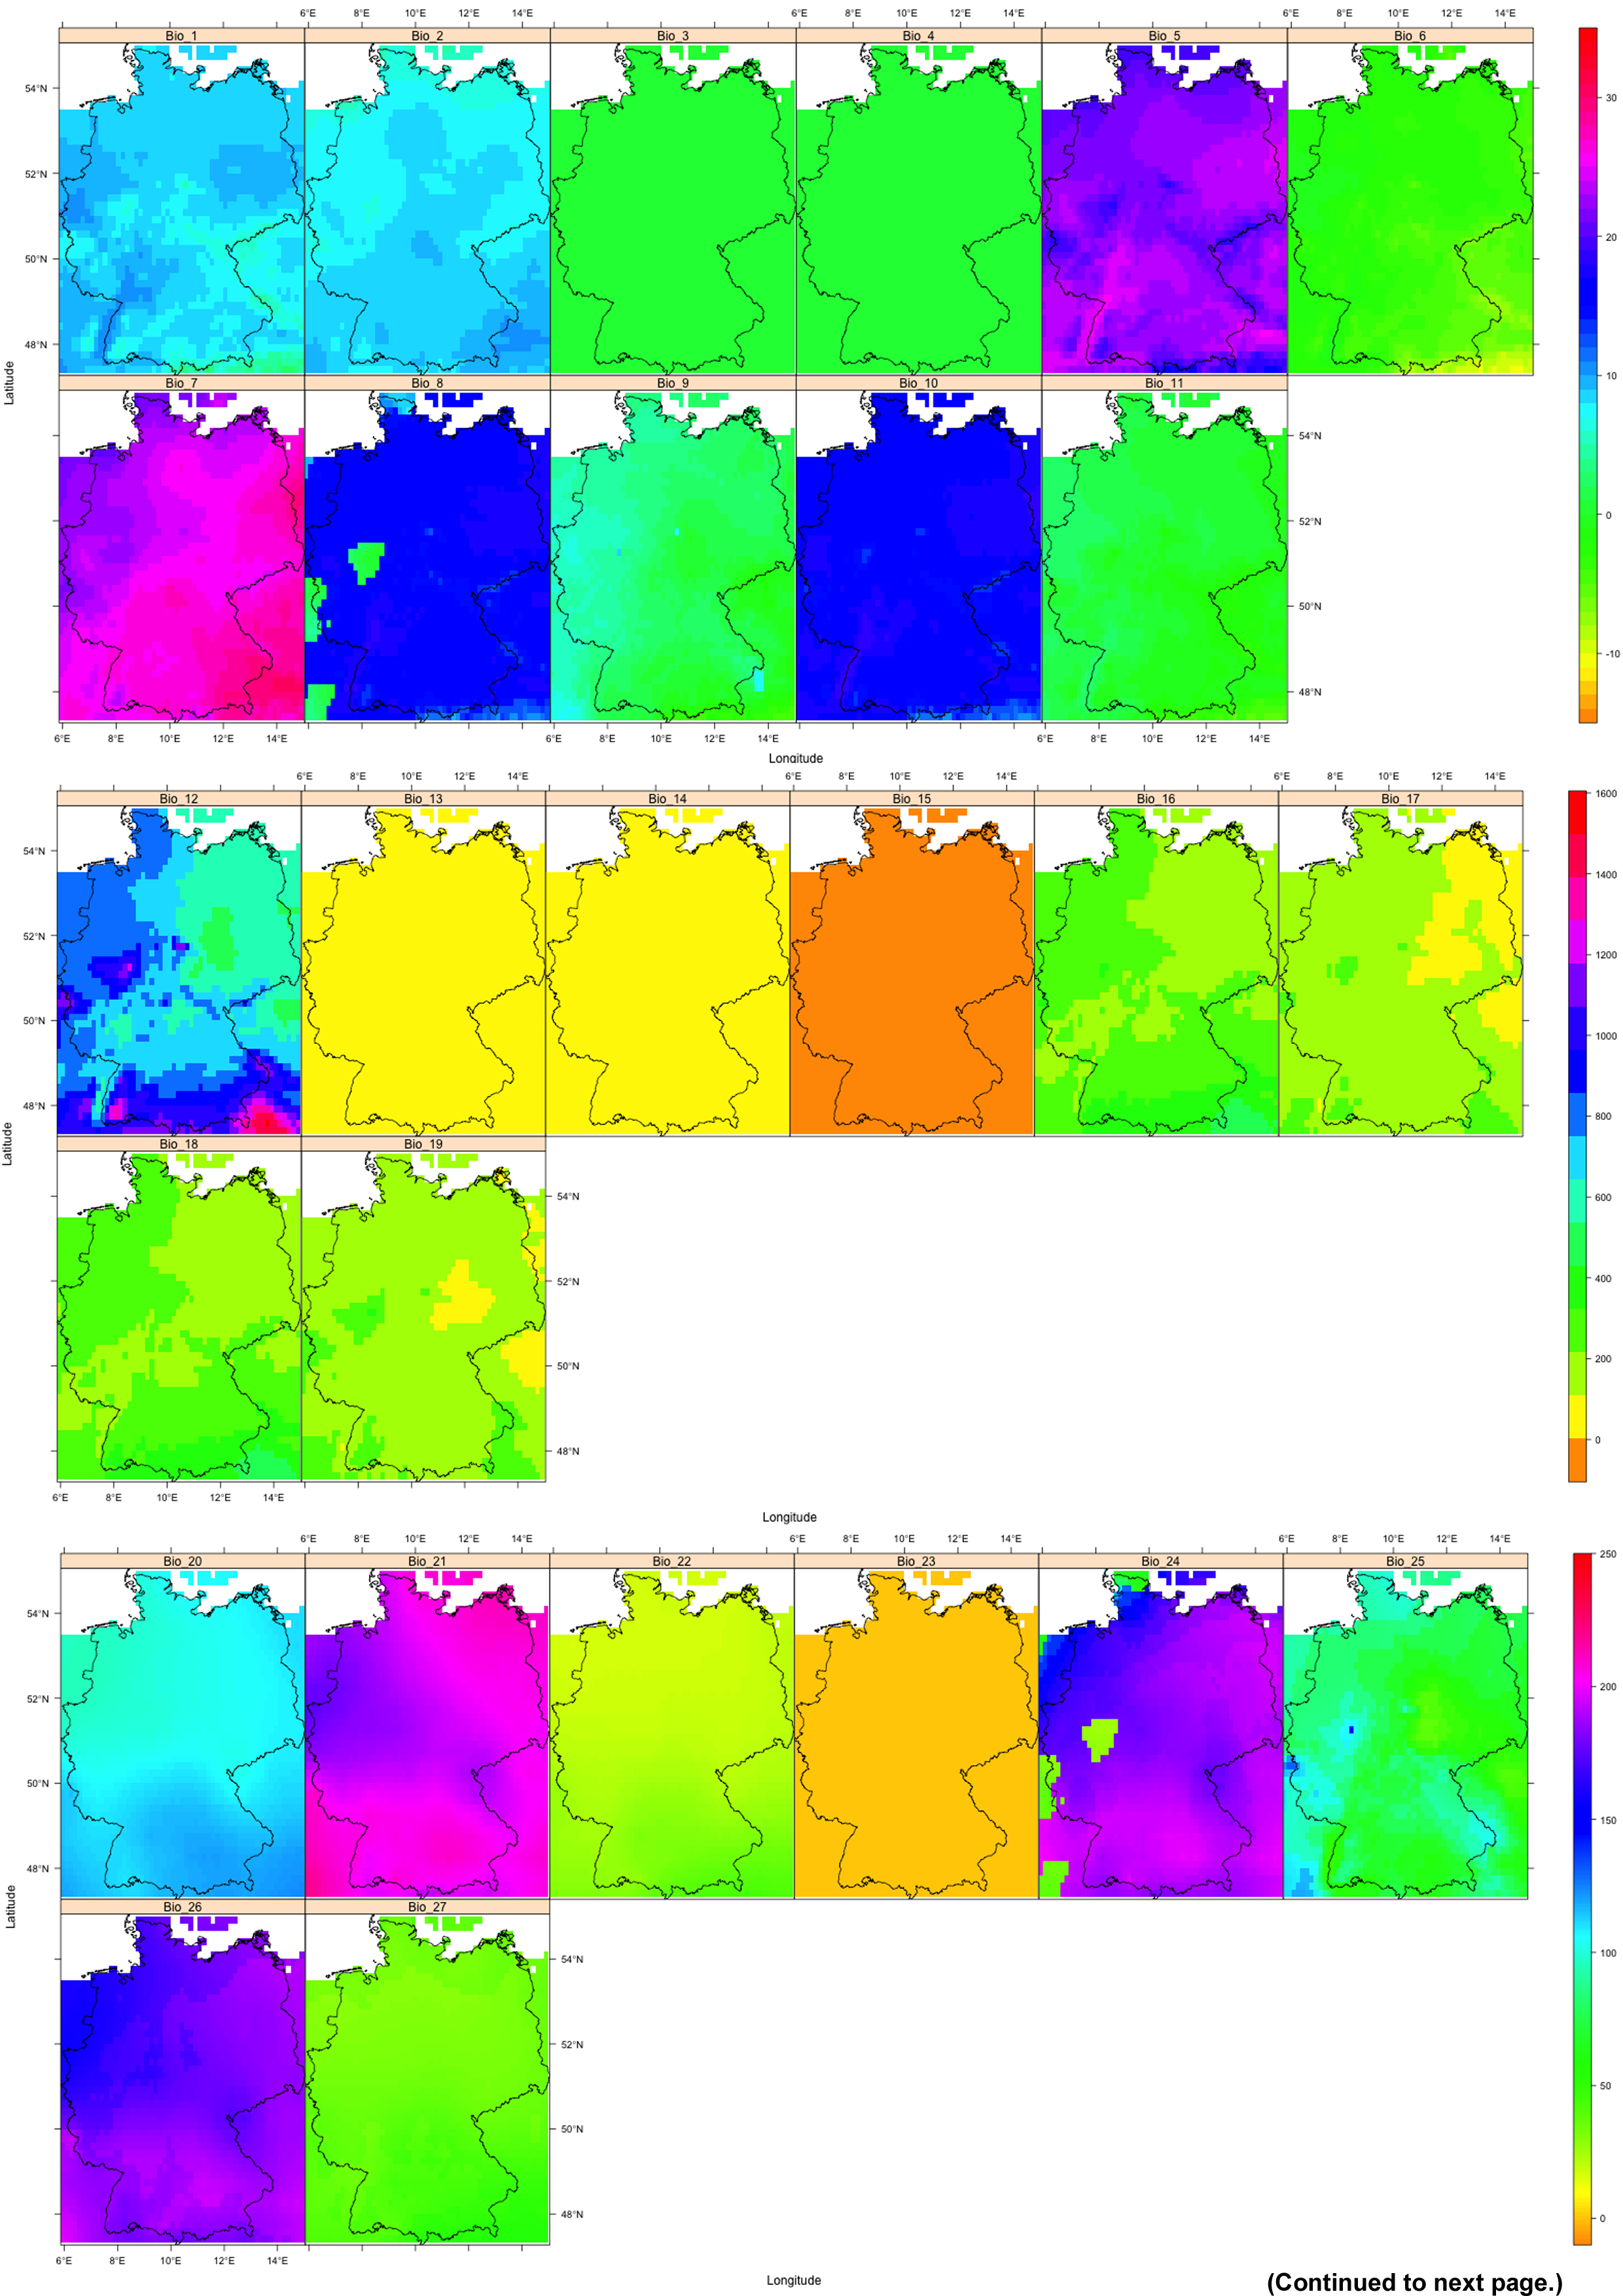
\includegraphics[width=1.1\textwidth]{Figures/Fig_C_2_a.png}
  \label{Fig_C_2_a}
\end{figure*}

\clearpage

\begin{figure}[h!]
  \centering
  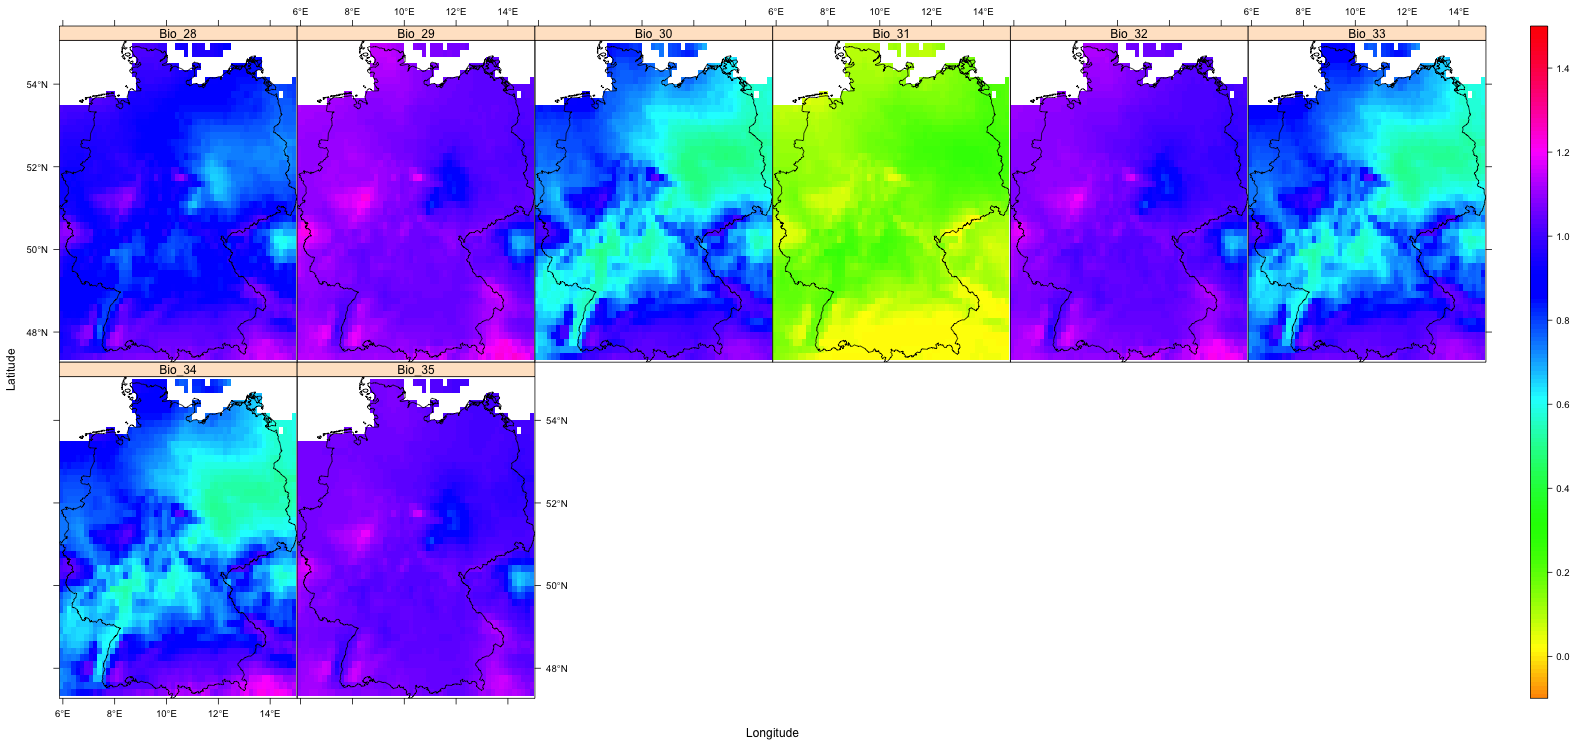
\includegraphics[width=\textwidth]{Figures/Fig_C_2_b.png}
  \caption{Extracted 35 global bioclimatic indices within the border of Germany. The indices are grouped according to their value ranges and units (\textsuperscript{0}C, mm, W m\textsuperscript{-2} and no unit). The panel captions indicate the IDs of the indices (Bio\textunderscore ID). Details on the indices and their IDs and units can be found in Table 2 and \href{https://www.climond.org/Resources.aspx}{https://www.climond.org/Resources.aspx}.}
  \label{Fig_C_2_b}
\end{figure}

\newpage

\begin{figure}[h!]
  \centering
  \captionsetup{width=1.1\textwidth}
  \hspace{-2cm}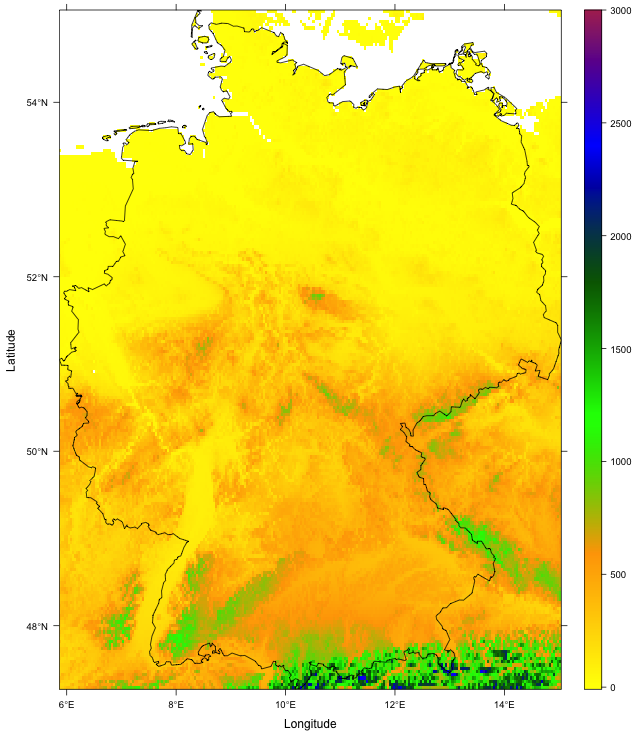
\includegraphics[width=1.1\textwidth]{Figures/Fig_C_3.png}
  \caption{Altitudes from the mean sea level (m) within the border of Germany. Details can be found in \href{http://asterweb.jpl.nasa.gov/gdem.asp}{http://asterweb.jpl.nasa.gov/gdem.asp}.}
  \label{Fig_C_3}
\end{figure}

\clearpage

\begin{figure}[hp!]
  \centering
  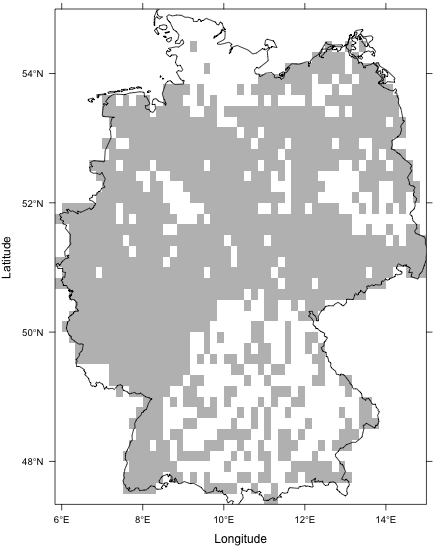
\includegraphics[width=\textwidth]{Figures/Fig_C_4.png}
  \caption{Bioclimatic indices (BIs) raster cells that are covered (72 \%) by the bio-monitoring steam sites.}
  \label{Fig_C_4}
\end{figure}

\clearpage

\begin{landscape}

\begin{figure}[h!]
  \centering
  \vspace{-2.3cm} 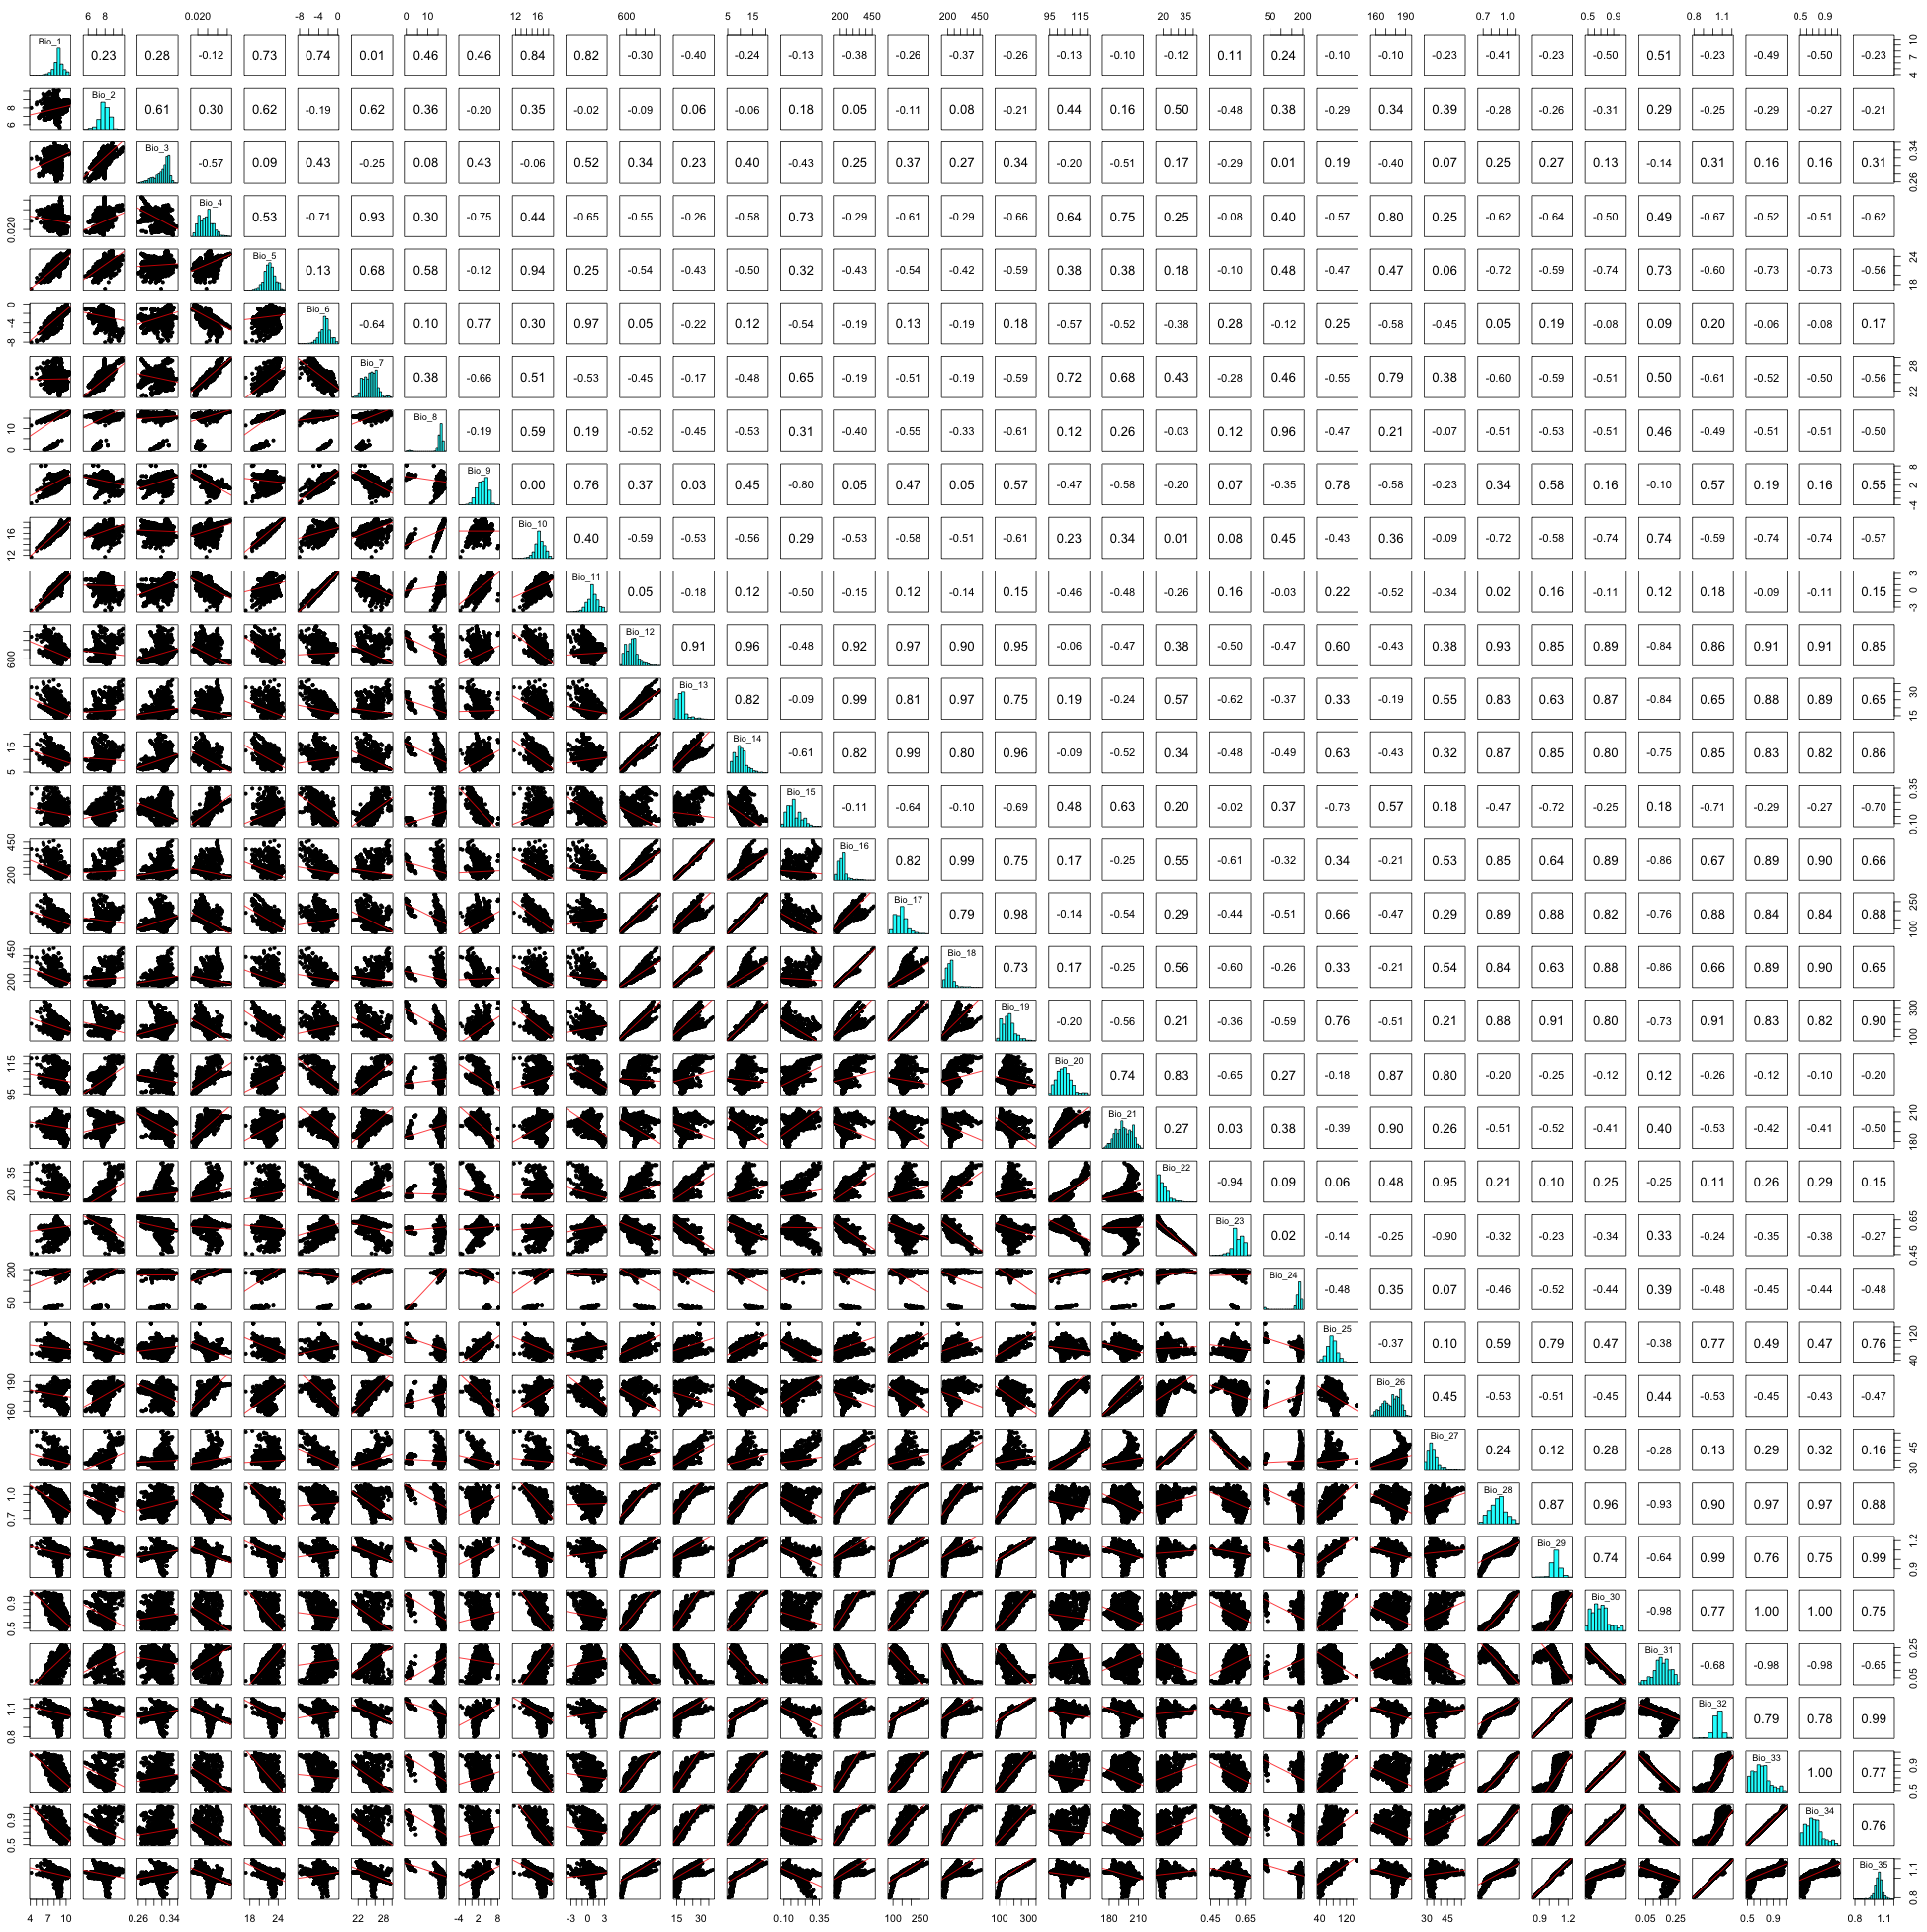
\includegraphics[width=1.2\textwidth]{Figures/Fig_C_5.png}
  \caption{Observed multicollinearity among the 35 bioclimatic indices (BIs). Statistically significant (p<0.001) pairwise correlation coefficients (Pearson) are reported with scatterplots and histograms showing distribution. Details on the indices and their IDs and units can be found in Table 2 and \href{https://www.climond.org/Resources.aspx}{https://www.climond.org/Resources.aspx}.}
  \label{Fig_C_5}
\end{figure}

\end{landscape}

\clearpage

\begin{figure}[h!]
  \centering
  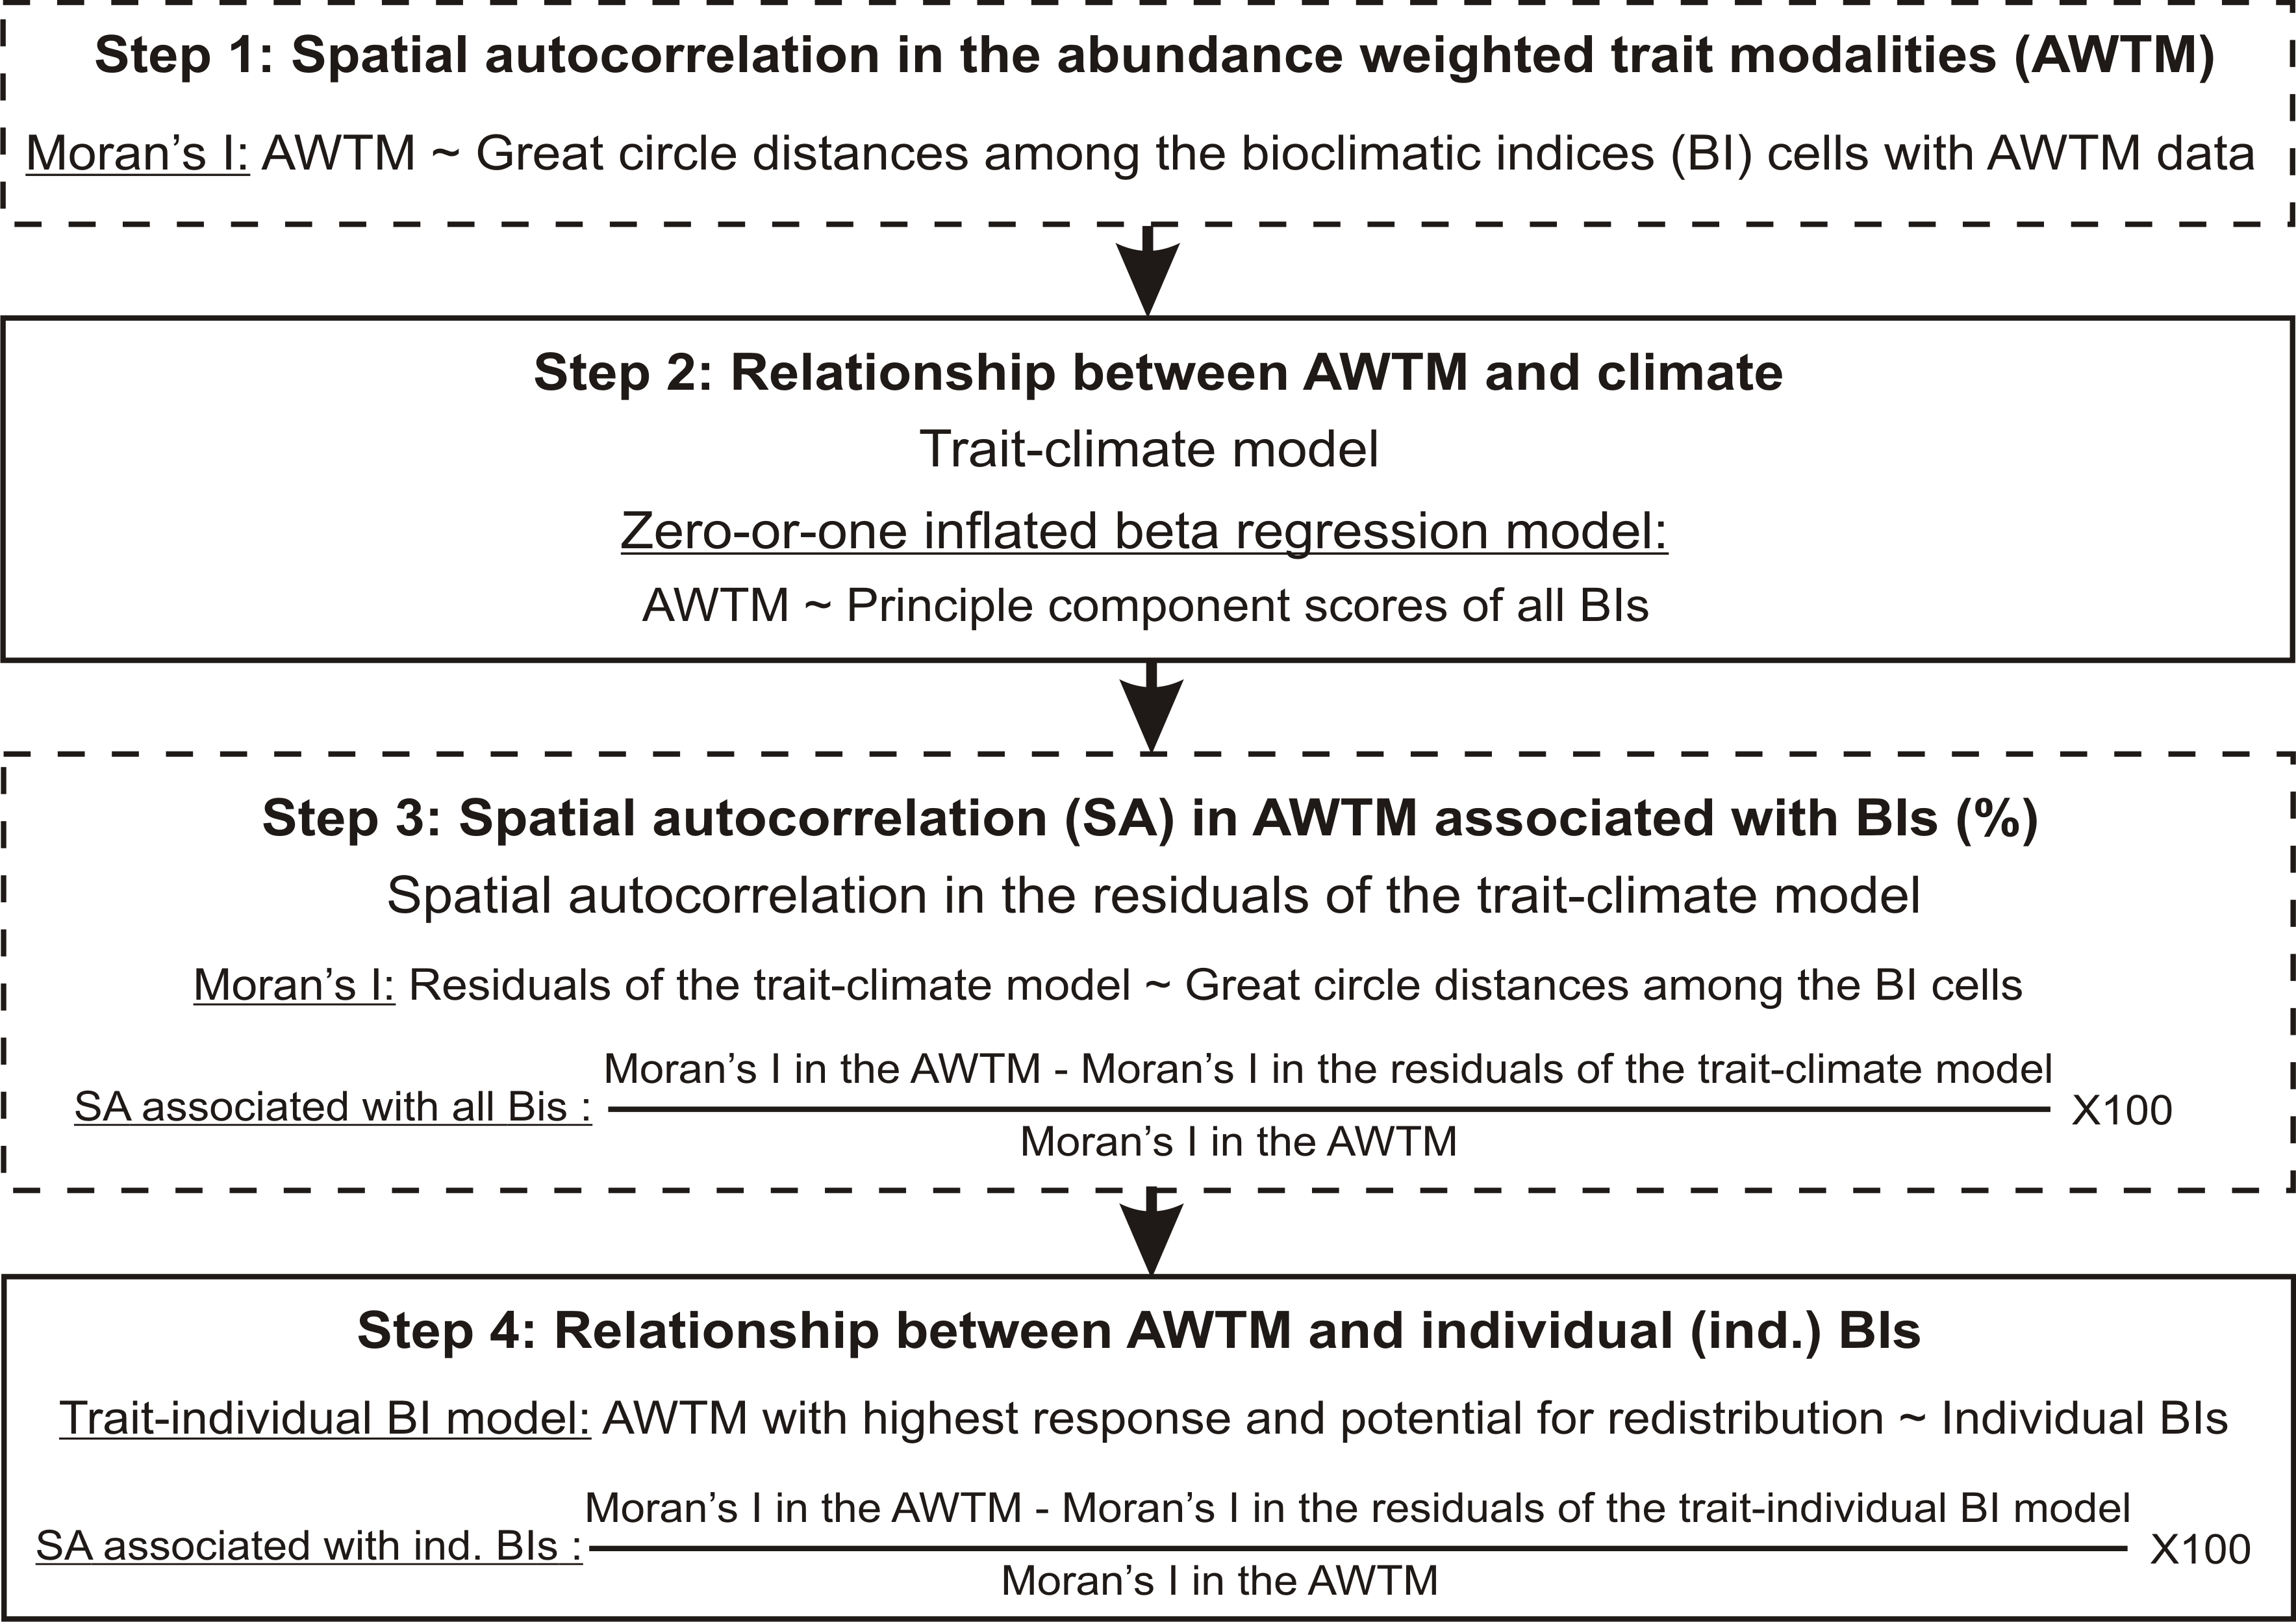
\includegraphics[width=1.1\textwidth]{Figures/Fig_C_6.png}
  \caption{Steps of the trait-climate spatial relationship analysis.}
  \label{Fig_C_6}
\end{figure}

\clearpage

\section{Supplementary tables}
\label{Supplementary tables}

\setlength{\LTcapwidth}{\linewidth}

\begin{longtable}[c]{>{\centering\arraybackslash}m{3.6cm}>{\centering\arraybackslash}m{1.3cm}>{\centering\arraybackslash}m{2.0cm}>{\centering\arraybackslash}m{1.3cm}>{\centering\arraybackslash}m{1.5cm}>{\centering\arraybackslash}m{1.5cm}}

\caption{Membership states of the five insect orders (\%) for the traits of each grouping feature. The membership state (\%) of an order for a trait was computed as the median of the membership states of all taxa in that order for that trait. The membership states were then scaled by the total of the membership states of an order for the traits of a grouping feature so that the membership states sum to 100 \% for each grouping feature.}

\centering

\hline
\textbf{Grouping features and traits} & \multicolumn{5}{c}{\textbf{Aquatic insect orders}}\\
 & \textbf{Diptera} & \textbf{Ephemeroptera} & \textbf{Odonata} & \textbf{Plecoptera} & \textbf{Trichoptera}\\
\hline
\endfirsthead

\hline
\endhead

\hline
\endfoot

\hline
\endlastfoot

\textbf{Biological traits} & & & & & \\
\textit{Dispersal capacity} & & & & & \\
Unknown & NA & NA & NA & NA & 9\\
Low & NA & 100* & NA & 100* & 36\\
High & NA & NA & NA & NA & 55*\\
\textit{Maximal body size} & & & & & \\
> 0.25 cm to 0.5 cm & 11 & 3 & NA & 6 & 11\\
> 0.5 cm to 1 cm & 39* & 43 & 3 & 39* & 37\\
> 1 cm to 2 cm & 29 & 50* & 44* & 36 & 39*\\
> 2 cm to 4 cm & 14 & 3 & 44* & 19 & 13\\
> 4 cm to 8 cm & 7 & NA & 9 & NA & NA\\
\textit{Reproductive capacity} & & & & & \\
Flexible & NA & 4 & NA & 7 & 5\\
Semivoltine & 4 & 2 & NA & 15 & 10\\
Univoltine & 39 & 64* & NA & 79* & 80*\\
Bivoltine & 44* & 23 & NA & NA & 4\\
Trivoltine & 11 & 5 & NA & NA & NA\\
Multivoltine & 3 & 1 & NA & NA & 1\\
\textit{Resistance to drought} & & & & & \\
Unknown resistance type & NA & NA & NA & 28 & 4\\
No drought resilience & NA & NA & NA & NA & 49*\\
Egg diapause & NA & 60* & NA & 62* & 3\\
Larvae diapause & NA & 40 & NA & 10 & 4\\
Adult diapause & NA & NA & NA & NA & 40\\
\textbf{Ecological traits} & & & & & \\
\textit{Current preference} & & & & & \\
Indifferent & 13 & NA & NA & 3 & 3\\
Limnobiont & 7 & 1 & 21 & NA & 19\\
Limnophil & 17 & 11 & 49* & 1 & 16\\
Limno to Rheophil & 4 & 10 & 14 & 2 & 12\\
Rheo to Limnophil & 14 & 27 & 7 & 10 & 13\\
Rheophil & 31* & 45* & 7 & 80* & 26*\\
Rheobiont & 13 & 7 & 3 & 5 & 11\\
\textit{Temperature preference} & & & & & \\
Eurytherm & 30* & 7 & NA & 1 & 48*\\
Very cold & 3 & 15 & NA & 16 & 6\\
Cold & 14 & 27 & NA & 46* & 14\\
Moderate & 26 & 32* & NA & 27 & 23\\
Warm & 27 & 19 & NA & 10 & 10\\

\end{longtable}

\vspace{-0.45cm}

\footnotesize
\textsuperscript{NA}Trait not occurring, *The highest membership state (\%) of an insect order for a trait in a grouping feature

\normalsize

\newpage

\begin{table}[hp!]

\label{Table C.2}

\caption{Spatial autocorrelations (Moran's I values) and gradients (Pearson correlations with longitude, latitude and altitude) for the bioclimatic indices (BIs) extracted at the stream sites. The Moran's I values and Pearson correlation coefficients are statistically significant at p<0.001. Details on the indices and their IDs and units can be found in Table 2 and \href{https://www.climond.org/Resources.aspx}{https://www.climond.org/Resources.aspx}.}

\centering

\begin{tabular}{>{\centering\arraybackslash}m{2.0cm}>{\centering\arraybackslash}m{2.0cm}>{\centering\arraybackslash}m{1.5cm}>{\centering\arraybackslash}m{1.5cm}>{\centering\arraybackslash}m{1.0cm}}

\toprule
\textbf{Bioclimatic indices} & \textbf{Spatial autocorrelation} & \multicolumn{3}{c}{\textbf{Correlation (Pearson) with spatial variables}}\\
\textbf{(BIs)} & \textbf{(Global Moran's I)} & & & \\
 & & \textbf{Longitude} & \textbf{Latitude} & \textbf{Altitude}\\

\midrule

Bio01 & 0.18 & -0.42 & 0.30 & -0.77\\
Bio02 & 0.29 & 0.16 & -0.77 & 0.52\\
Bio03 & 0.28 & -0.54 & -0.53 & 0.26\\
Bio04 & 0.36 & 0.86 & -0.34 & 0.30\\
Bio05 & 0.13 & 0.10 & -0.20 & -0.32\\
Bio06 & 0.32 & -0.68 & 0.49 & -0.76\\
Bio07 & 0.34 & 0.68 & -0.58 & 0.45\\
Bio08 & 0.09 & 0.28 & 0.13 & -0.3\\
Bio09 & 0.30 & -0.75 & 0.33 & -0.58\\
Bio10 & 0.12 & 0.00 & 0.15 & -0.64\\
Bio11 & 0.30 & -0.70 & 0.40 & -0.73\\
Bio12 & 0.27 & -0.27 & -0.58 & 0.69\\
Bio13 & 0.30 & 0.04 & -0.67 & 0.80\\
Bio14 & 0.26 & -0.45 & -0.55 & 0.60\\
Bio15 & 0.30 & 0.72 & -0.28 & 0.33\\
Bio16 & 0.30 & 0.03 & -0.66 & 0.79\\
Bio17 & 0.25 & -0.44 & -0.51 & 0.59\\
Bio18 & 0.30 & 0.05 & -0.66 & 0.79\\
Bio19 & 0.24 & -0.53 & -0.39 & 0.47\\
Bio20 & 0.38 & 0.36 & -0.78 & 0.68\\
Bio21 & 0.29 & 0.43 & -0.23 & 0.11\\
Bio22 & 0.40 & 0.16 & -0.89 & 0.84\\
Bio23 & 0.41 & -0.09 & 0.92 & -0.86\\
Bio24 & 0.13 & 0.43 & -0.14 & 0.08\\
Bio25 & 0.20 & -0.53 & 0.02 & 0.04\\
Bio26 & 0.33 & 0.53 & -0.51 & 0.35\\
Bio27 & 0.37 & 0.25 & -0.78 & 0.83\\
Bio28 & 0.24 & -0.33 & -0.37 & 0.56\\
Bio29 & 0.19 & -0.48 & -0.13 & 0.29\\
Bio30 & 0.25 & -0.09 & -0.46 & 0.67\\
Bio31 & 0.26 & 0.06 & 0.47 & -0.64\\
Bio32 & 0.20 & -0.51 & -0.16 & 0.31\\
Bio33 & 0.25 & -0.14 & -0.47 & 0.66\\
Bio34 & 0.25 & -0.12 & -0.48 & 0.69\\
Bio35 & 0.20 & -0.51 & -0.21 & 0.30\\

\bottomrule

\end{tabular}
\end{table}

\newpage

\setlength{\LTcapwidth}{\linewidth}

\begin{longtable}[c]{>{\centering\arraybackslash}m{3.6cm}>{\centering\arraybackslash}m{1.0cm}>{\centering\arraybackslash}m{2.0cm}>{\centering\arraybackslash}m{1.0cm}>{\centering\arraybackslash}m{1.2cm}>{\centering\arraybackslash}m{1.2cm}>{\centering\arraybackslash}m{1.2cm}}

\caption{Spatial autocorrelations (global Moran's I) for abundance weighted traits in each stream macroinvertebrate order and in the full data. Observed Moran's I values are statistically significant at p<0.001.}

\centering

\hline
\textbf{Grouping features and traits} & \multicolumn{5}{c}{\textbf{Aquatic insect orders}} & \textbf{Full data}\\
 & \textbf{Diptera} & \textbf{Ephemeroptera} & \textbf{Odonata} & \textbf{Plecoptera} & \textbf{Trichoptera} & \\
\hline
\endfirsthead

\hline
\endhead

\hline
\endfoot

\hline
\textbf{\textit{Average over traits and orders}} & \textbf{\textit{0.06}} & \textbf{\textit{0.06}} & \textbf{\textit{0.07}} & \textbf{\textit{0.09}} & \textbf{\textit{0.05}} & \textbf{\textit{0.06}}\\
\hline
\endlastfoot

\textbf{Biological traits} & & & & & & \\
\textit{Dispersal capacity} & & & & & & \\
Unknown & NA & NA & NA & NA & 0.05 & 0.03\\
Low & NA & * & NA & * & 0.03 & 0.04\\
High & NA & NA & NA & NA & 0.02 & 0.03\\
\textit{Average} & \textit{NA} & \textit{NA} & \textit{NA} & \textit{NA} & \textit{0.03} & \textit{0.03}\\
\textit{Maximal body size} & & & & & & \\
> 0.25 cm to 0.5 cm & 0.02 & 0.04 & NA & 0.12 & 0.03 & 0.04\\
> 0.5 cm to 1 cm & 0.03 & 0.02 & NA & 0.03 & 0.03 & 0.03\\
> 1 cm to 2 cm & 0.02 & 0.04 & 0.13 & 0.15 & 0.03 & 0.03\\
> 2 cm to 4 cm & 0.04 & 0.03 & 0.06 & 0.04 & 0.03 & 0.03\\
> 4 cm to 8 cm & 0.02 & NA & 0.08 & NA & NA & 0.04\\
\textit{Average} & \textit{0.03} & \textit{0.03} & \textit{0.09} & \textit{0.09} & \textit{0.03} & \textit{0.03}\\
\textit{Reproductive capacity} & & & & & & \\
Flexible & NA & 0.07 & NA & 0.08 & 0.02 & 0.03\\
Semivoltine & 0.03 & 0.03 & NA & 0.03 & 0.08 & 0.02\\
Univoltine & 0.12 & 0.03 & NA & 0.04 & 0.07 & 0.04\\
Bivoltine & 0.12 & 0.03 & NA & NA & 0.04 & 0.05\\
Trivoltine & 0.06 & 0.10 & NA & NA & NA & 0.04\\
Multivoltine & 0.05 & 0.08 & NA & NA & 0.01 & 0.03\\
\textit{Average} & \textit{0.08} & \textit{0.06} & \textit{NA} & \textit{0.05} & \textit{0.04} & \textit{0.04}\\
\textit{Resistance to drought} & & & & & & \\
Unknown resistance type & NA & NA & NA & 0.19 & 0.02 & 0.03\\
No drought resilience & NA & NA & NA & NA & 0.10 & 0.04\\
Egg diapause & NA & 0.08 & NA & 0.2 & 0.01 & 0.12\\
Larvae diapause & NA & 0.08 & NA & 0.00 & 0.01 & 0.17\\
Adult diapause & NA & NA & NA & NA & 0.13 & 0.02\\
\textit{Average} & \textit{NA} & \textit{0.08} & \textit{NA} & \textit{0.13} & \textit{0.05} & \textit{0.08}\\
\textbf{Ecological traits} & & & & & & \\
\textit{Current preference} & & & & & & \\
Indifferent & 0.10 & NA & NA & 0.03 & 0.02 & 0.08\\
Limnobiont & 0.01 & NA & 0.02 & NA & 0.10 & 0.07\\
Limnophil & 0.05 & 0.13 & 0.08 & 0.17 & 0.16 & 0.14\\
Limno to Rheophil & 0.07 & 0.01 & 0.10 & 0.02 & 0.04 & 0.02\\
Rheo to Limnophil & 0.04 & 0.07 & 0.04 & 0.00 & 0.01 & 0.03\\
Rheophil & 0.09 & 0.05 & 0.11 & 0.20 & 0.11 & 0.13\\
Rheobiont & 0.06 & 0.07 & 0.05 & 0.06 & 0.13 & 0.15\\
\textit{Average} & \textit{0.06} & \textit{0.07} & \textit{0.07} & \textit{0.08} & \textit{0.08} & \textit{0.09}\\
\textit{Temperature preference} & & & & & & \\
Eurytherm & 0.08 & 0.08 & NA & 0.15 & 0.05 & 0.10\\
Very cold & 0.06 & 0.11 & NA & 0.14 & 0.06 & 0.15\\
Cold & 0.08 & 0.03 & NA & 0.10 & 0.07 & 0.13\\
Moderate & 0.03 & 0.09 & NA & 0.08 & 0.01 & 0.01\\
Warm & 0.07 & 0.03 & NA & 0.09 & 0.05 & 0.06\\
\textit{Average} & \textit{0.06} & \textit{0.07} & \textit{NA} & \textit{0.11} & \textit{0.05} & \textit{0.09}\\

\end{longtable}

\vspace{-0.4cm}

\footnotesize
\textsuperscript{NA}Trait not occurring\\
\hspace{0.4cm} *Trait omitted from the analysis because of zero variability (i.e. all taxa have same trait) and therefore the abundance weighted trait cannot be computed\\

\normalsize

\clearpage

\begin{table}[hp!]

\label{Table C.4}

\caption{Relationship between the traits of temperature preference grouping feature and the traits of remaining grouping features in terms of explained variance (\%). The explained variances are the $R^2$s of the zero-or-one-inflated beta regression models fitted with the abundance weighted traits (AWT) of the temperature preference grouping feature as response and the AWT of the remaining grouping features separately as predictor variables.}

\centering

\begin{threeparttable}

\begin{tabular}{>{\centering\arraybackslash}m{3.6cm}>{\centering\arraybackslash}m{1.3cm}>{\centering\arraybackslash}m{1.4cm}>{\centering\arraybackslash}m{1.0cm}>{\centering\arraybackslash}m{1.3cm}>{\centering\arraybackslash}m{1.0cm}}

\toprule
\textbf{Remaining grouping features and traits} & \multicolumn{5}{c}{\textbf{Traits of temperature preference grouping feature}}\\
 & \textbf{Eurytherm} & \textbf{Very cold} & \textbf{Cold} & \textbf{Moderate} & \textbf{Warm}\\

\midrule

\textbf{Biological traits} & & & & & \\
\textit{Dispersal capacity} & & & & & \\
Unknown & 3.6* & 0.1 & 2.0 & 0.0 & 0.0\\
Low & 3.2 & 1.2* & 9.8* & 1.5* & 15\\
High & 0.9 & 0.5 & 4.5 & 1.4 & 17*\\
\textit{Maximal body size} & & & & & \\
> 0.25 cm to 0.5 cm & 2.0 & 10 & 2.8 & 3.4* & 2.1*\\
> 0.5 cm to 1 cm & 1.9 & 0.0 & 1.8 & 0.4 & 0.6\\
> 1 cm to 2 cm & 4.4 & 10 & 4.3 & 0.2 & 1.7\\
> 2 cm to 4 cm & 5.7* & 0.0 & 2.7 & 1.1 & 0.1\\
> 4 cm to 8 cm & 3.2 & 13* & 5.8* & 0.3 & 1.9\\
\textit{Reproductive capacity} & & & & & \\
Flexible & 1.6 & 3.2 & 1.1 & 9.7 & 3.2\\
Semivoltine & 0.1 & 9.0 & 16* & 1.7 & 16\\
Univoltine & 2.9 & 15* & 7.5 & 4.2 & 6.7\\
Bivoltine & 2.7 & 1.0 & 4.5 & 0.0 & 0.8\\
Trivoltine & 0.7 & 7.0 & 1.3 & 10 & 0.8\\
Multivoltine & 1.7 & 15 & 0.1 & 14* & 36*\\
\textit{Resistance to drought} & & & & & \\
Unknown resistance type & 1.8 & 6.2 & 0.3 & 1.8 & 11\\
No drought resilience & 6.7 & 2.8 & 6.3 & 0.0 & 0.3\\
Egg diapause & 28* & 13 & 30* & 1.4 & 6.6\\
Larvae diapause & 0.0 & 25* & 0.7 & 0.0 & 0.6\\
Adult diapause & 15 & 0.0 & 16 & 3.7* & 14*\\
\textbf{Ecological traits} & & & & & \\
\textit{Current preference} & & & & & \\
Indifferent & 13 & 36 & 30 & 0.9 & 12*\\
Limnobiont & 12 & 14 & 16 & 0.6 & 0.8\\
Limnophil & 18 & 41 & 27 & 1.3* & 4.6\\
Limno to Rheophil & 0.5 & 1.6 & 0.7 & 0.1 & 0.0\\
Rheo to Limnophil & 3.0 & 0.0 & 0.0 & 0.6 & 0.0\\
Rheophil & 26* & 42* & 35* & 0.2 & 2.6\\
Rheobiont & 5.3 & 16 & 12 & 0.8 & 6.6\\

\bottomrule

\end{tabular}
\begin{tablenotes}
\footnotesize
* The highest explained variance in the traits of the temperature preference grouping feature by the traits of the remaining grouping features
\end{tablenotes}
\end{threeparttable}
\end{table}